% \documentclass[12pt,journal,compsoc]{IEEEtran}
\documentclass[10pt,journal,compsoc]{IEEEtran}
\usepackage{graphicx}

\ifCLASSOPTIONcompsoc
\else
\fi

\ifCLASSINFOpdf
\else
\fi

\newcommand\MYhyperrefoptions{
bookmarks=true,bookmarksnumbered=true,
pdfpagemode={UseOutlines},plainpages=false,pdfpagelabels=true,
colorlinks=true,linkcolor={black},citecolor={black},urlcolor={black},
pdftitle={Rancang Bangun Robot Vision Untuk Object Finding Menggunakan Color Tracking pada perangkat RaspberryPi},
pdfsubject={Typesetting},
pdfauthor={Achmadi},
pdfkeywords={Kata Kunci}
}

\begin{document}


 \title{Rancang Bangun Robot Vision Untuk Object Finding Menggunakan Color Tracking pada perangkat RaspberryPi}

 \author{
  Achmadi,2410100085
 \thanks{Dicetak 10 Desember 2014}
 }
 
 \markboth{Handout Progres 1 TA Gasal 2014}{RapberryPi RoboVision}
 
%   \IEEEtitleabstractindextext{
%   
%   \begin{abstract}
%   Ini Abstrak.
%   \end{abstract}
%   
%   \begin{IEEEkeywords}
%   Ini Kata Kunci
%   \end{IEEEkeywords}
%   }
  
  \maketitle
  
  \IEEEdisplaynontitleabstractindextext
  \IEEEpeerreviewmaketitle
 
 \section{Pendahuluan}
  \IEEEPARstart{R}{obot} vision adalah robot yang mampu menggunakan kamera sebagai sumber informasi untuk diolah sesuai kebutuhan. 
  Tujuan utama setiap perancangan robot tentu adalah untuk mengganti pekerjaan manusia. 
  Kemampuan robot untuk melakukan pekerjaan yang berulang dan berbahaya telah menjadi kebutuhan di setiap lingkungan industri.
  Untuk memenuhi kebutuhan tersebut telah dikembangkan beragam teknologi sensor dan actuator. 
  Khusus untuk sensor, telah dikembangkan teknologi yang mirip dengan cara kerja pada indra manusia. 
  Salah satu yang banyak dipakai adalah penggunaan kamera sebagai pengganti mata untuk robot.
  Penggunaan kamera sebagai sensor visual telah banyak di terapkan pada bidang robotika.
  RaspberryPi merupakan salah satu jenis SBC (Single Board Computer) dengan spesifikasi processor BCM235 arsitektur arm1176 kategori armhf dan RAM 512. 
  Tersedia Operating System yang dapat dijalankan oleh RaspberryPi yaitu Raspbian yang berbasis Linux dan memiliki pustaka pengolahan citra OpenCV di lumbung perangkat lunaknya. 
  RaspberryPi dan Operating System Raspbian merupakan proyek opensource yang bersifat gratis.
  Pustaka OpenCV (Open Computer Vision) merupakan pustaka pemrograman berbasis C/C++/Python yang berisi fungsi-fungsi untuk akuisisi dan pengolahan citra.
  Penjejakan warna merupakan salah satu bentuk pengenalan objek yang cukup sederhana. 
  Prinsip proses penjejakan warna adalah mensegmentasi gambar sesuai warna kemudian membaca perubahan distribusi pixel hasil segmentasi.
  Mode warna HSV adalah mode warna yang menyatakan warna dalam 3 variabel yaitu Hue, Saturation, dan Value.
  Nilai Hue merepresentasikan nilai jenis warna yang merupakan nilai kombinasi RGB dalam besaran sudut. 
  Pada dasarnya nilai Hue dibagi dalam juring lingkaran sehingga jangkauan nilainya adalah 0-360, 
  namun karena dalam bahasa pemrograman variabel pemrograman hanya 8bit (0-255) maka jangkauan juring di reduksi menjadi setengah lingkaran (0-179).
  Segmentasi citra adalah proses mengumpulkan pixel-pixel karena kesamaan properti. 
  Kesamaan properti dapat berupa nilai intensitas, bentuk tekstur,garis tepi, dll. 
  Ada banyak teknik untuk segmentasi citra dengan masing-masing memiliki kompleksitas, kemampuan, dan penggunaannya.
  Proses segmentasi merupakan proses yang penting dalam pengolahan citra.
  Segmentasi digunakan untuk memfilter objek yang tidak dibutuhkan. 
  Filter dapat berupa persamaan matematis,logic maupun maupun matrix kernel.
  
  \section{Metode Penelitian}
  
  \subsection{Alur Penelitian}
  Pada penelitian tugas akhir ini langkah awal yang dilakukan adalah studi literatur. 
  Studi literatur ini digunakan untuk mendapatkan referensi mengenai skema peralatan dan perancangan eksperimen yang sesuai. 
  Langkah selanjutnya adalah pembuatan robot berdasarkan literatur atau design yang telah ada.
  Langkah selanjutnya adalah mendapatkan data robot tersebut untuk menentukan nilai tresholding. 
  Langkah selanjutnya adalah menguji robot apakah mampu menemukan objek atau tidak.
  Jika tidak mammpu menemukan objek maka dilakukan penetuan penilai tresholding.
  Selanjutnya langkah terakhir adalah penulisan laporan.
  Berikut adalah flowchart :
  \begin{center}
    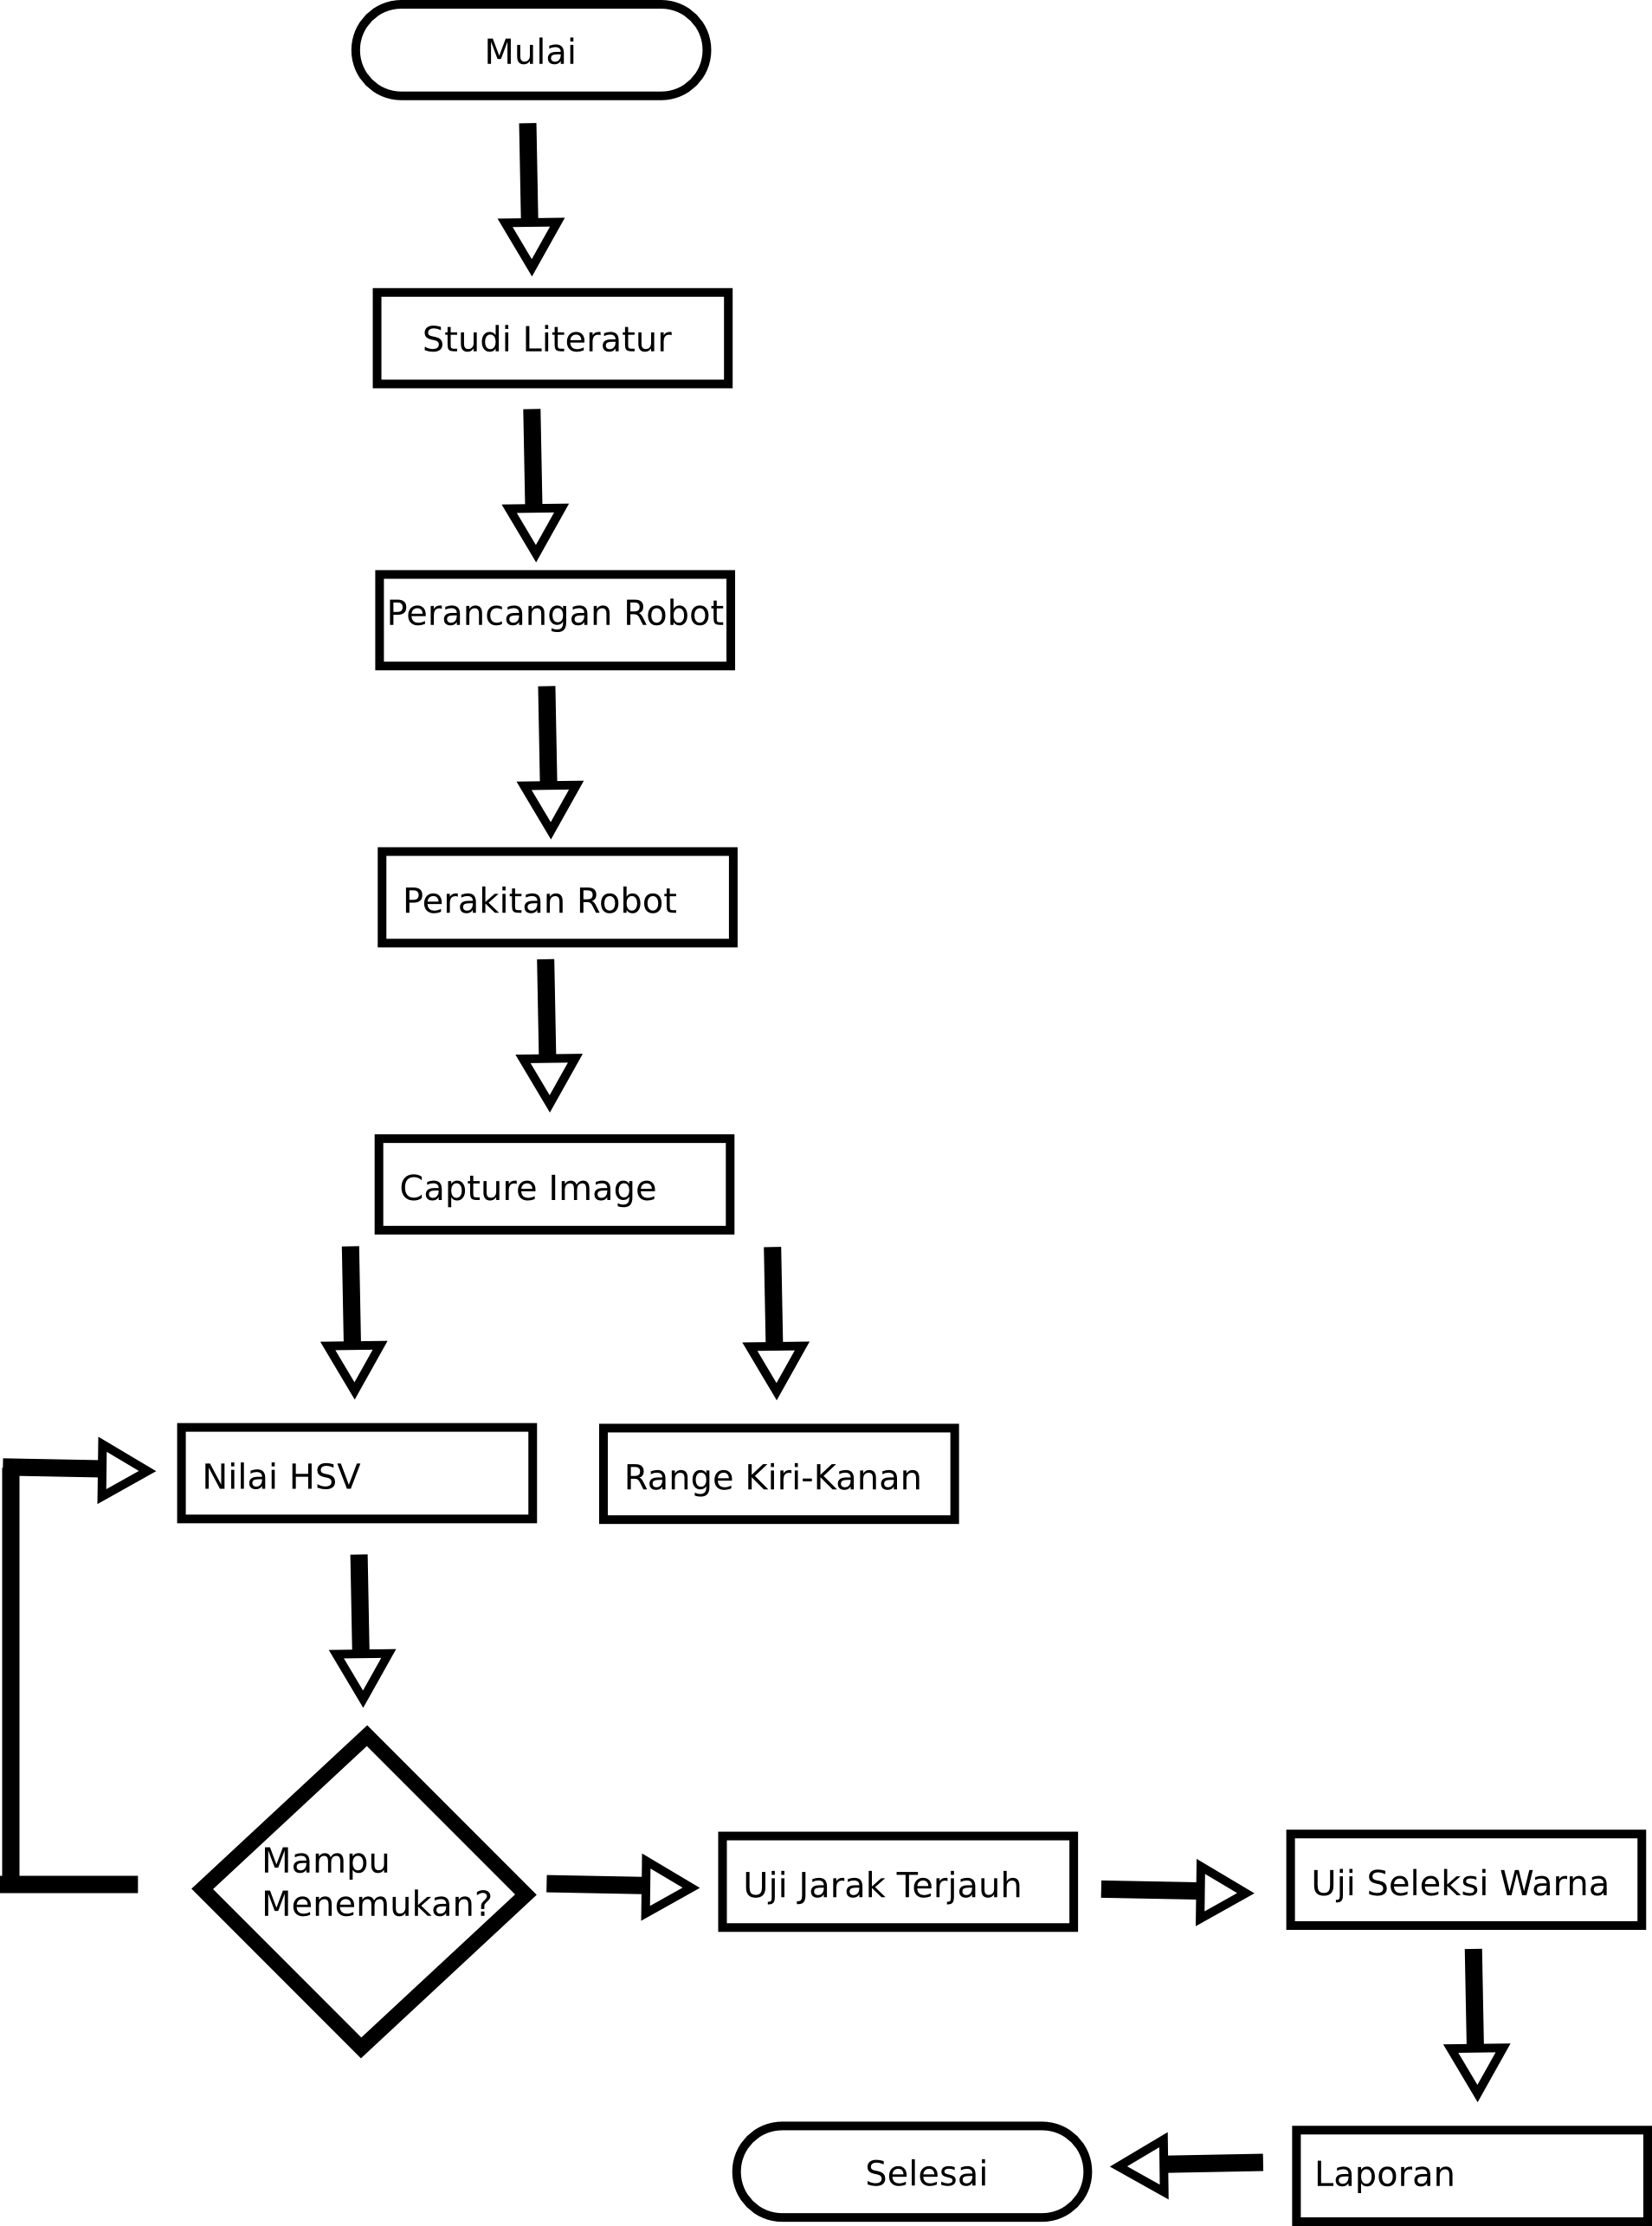
\includegraphics[width=120pt]{work}\\
  \end{center}
  
  \subsection{Perancangan Alat}
  Secara global robot ini terdiri dari:\\
  - RaspberrPi sebagai CPU untuk pengolahan Citra\\
  - Kamera sebagai Input\\
  - Motor Controller\\
  - Motor Driver\\
  - Motor DC Geared\\
  - LiPo Battery (5v an 12v)\\
  - Box \\
  
  \begin{center}
    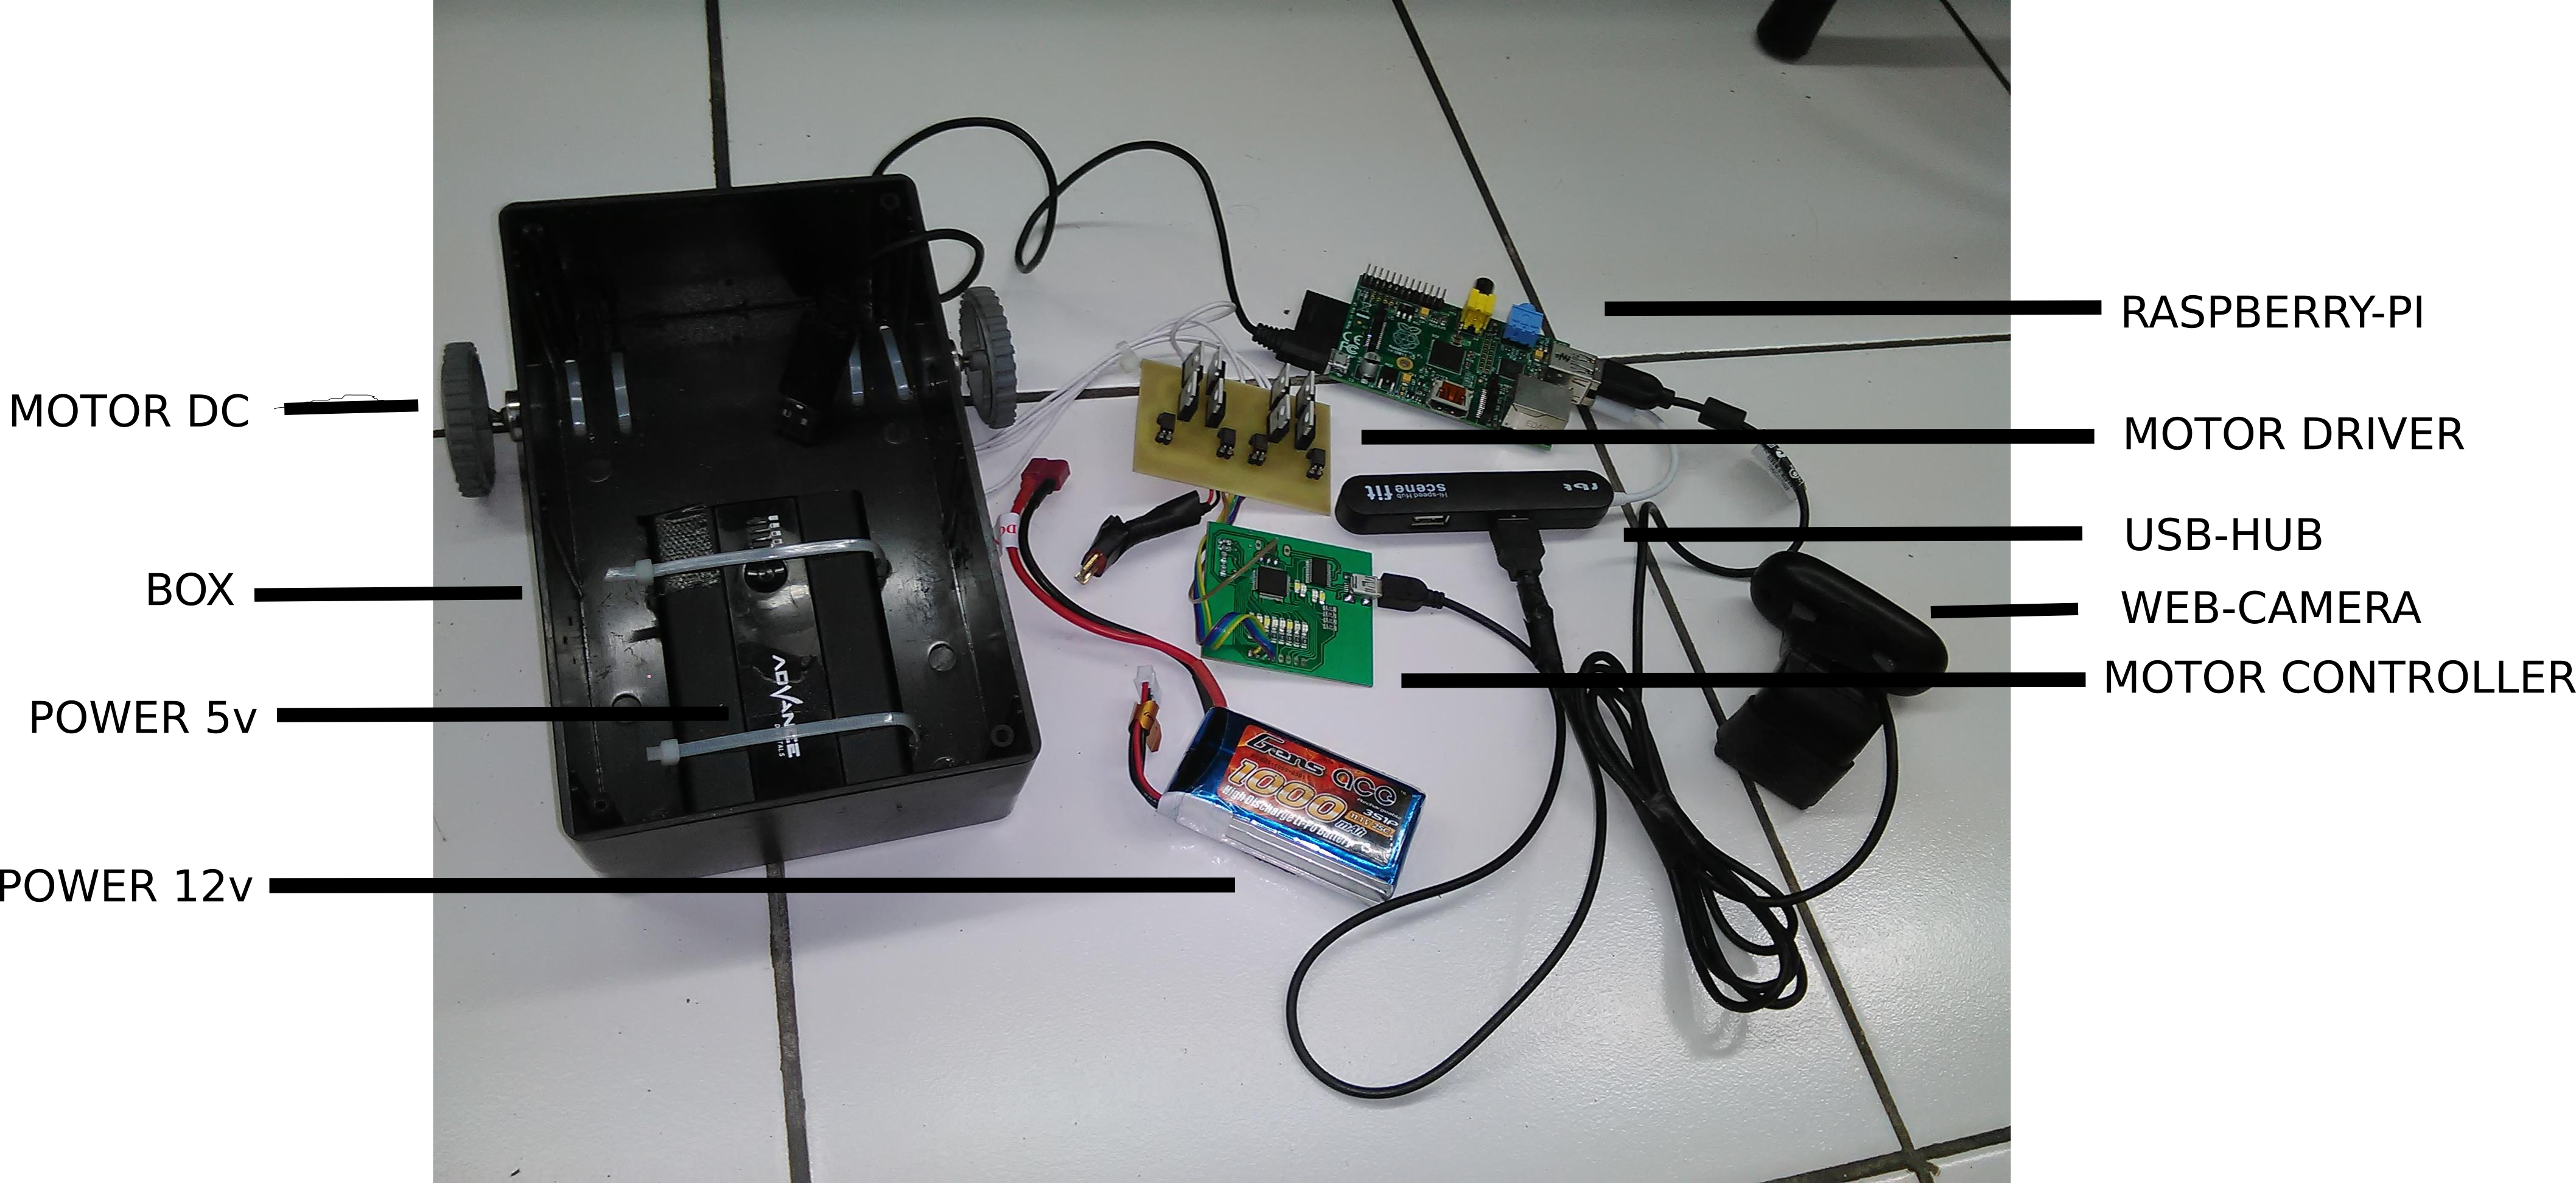
\includegraphics[width=200pt]{appart}\\
  \end{center}
  
  \begin{center}
    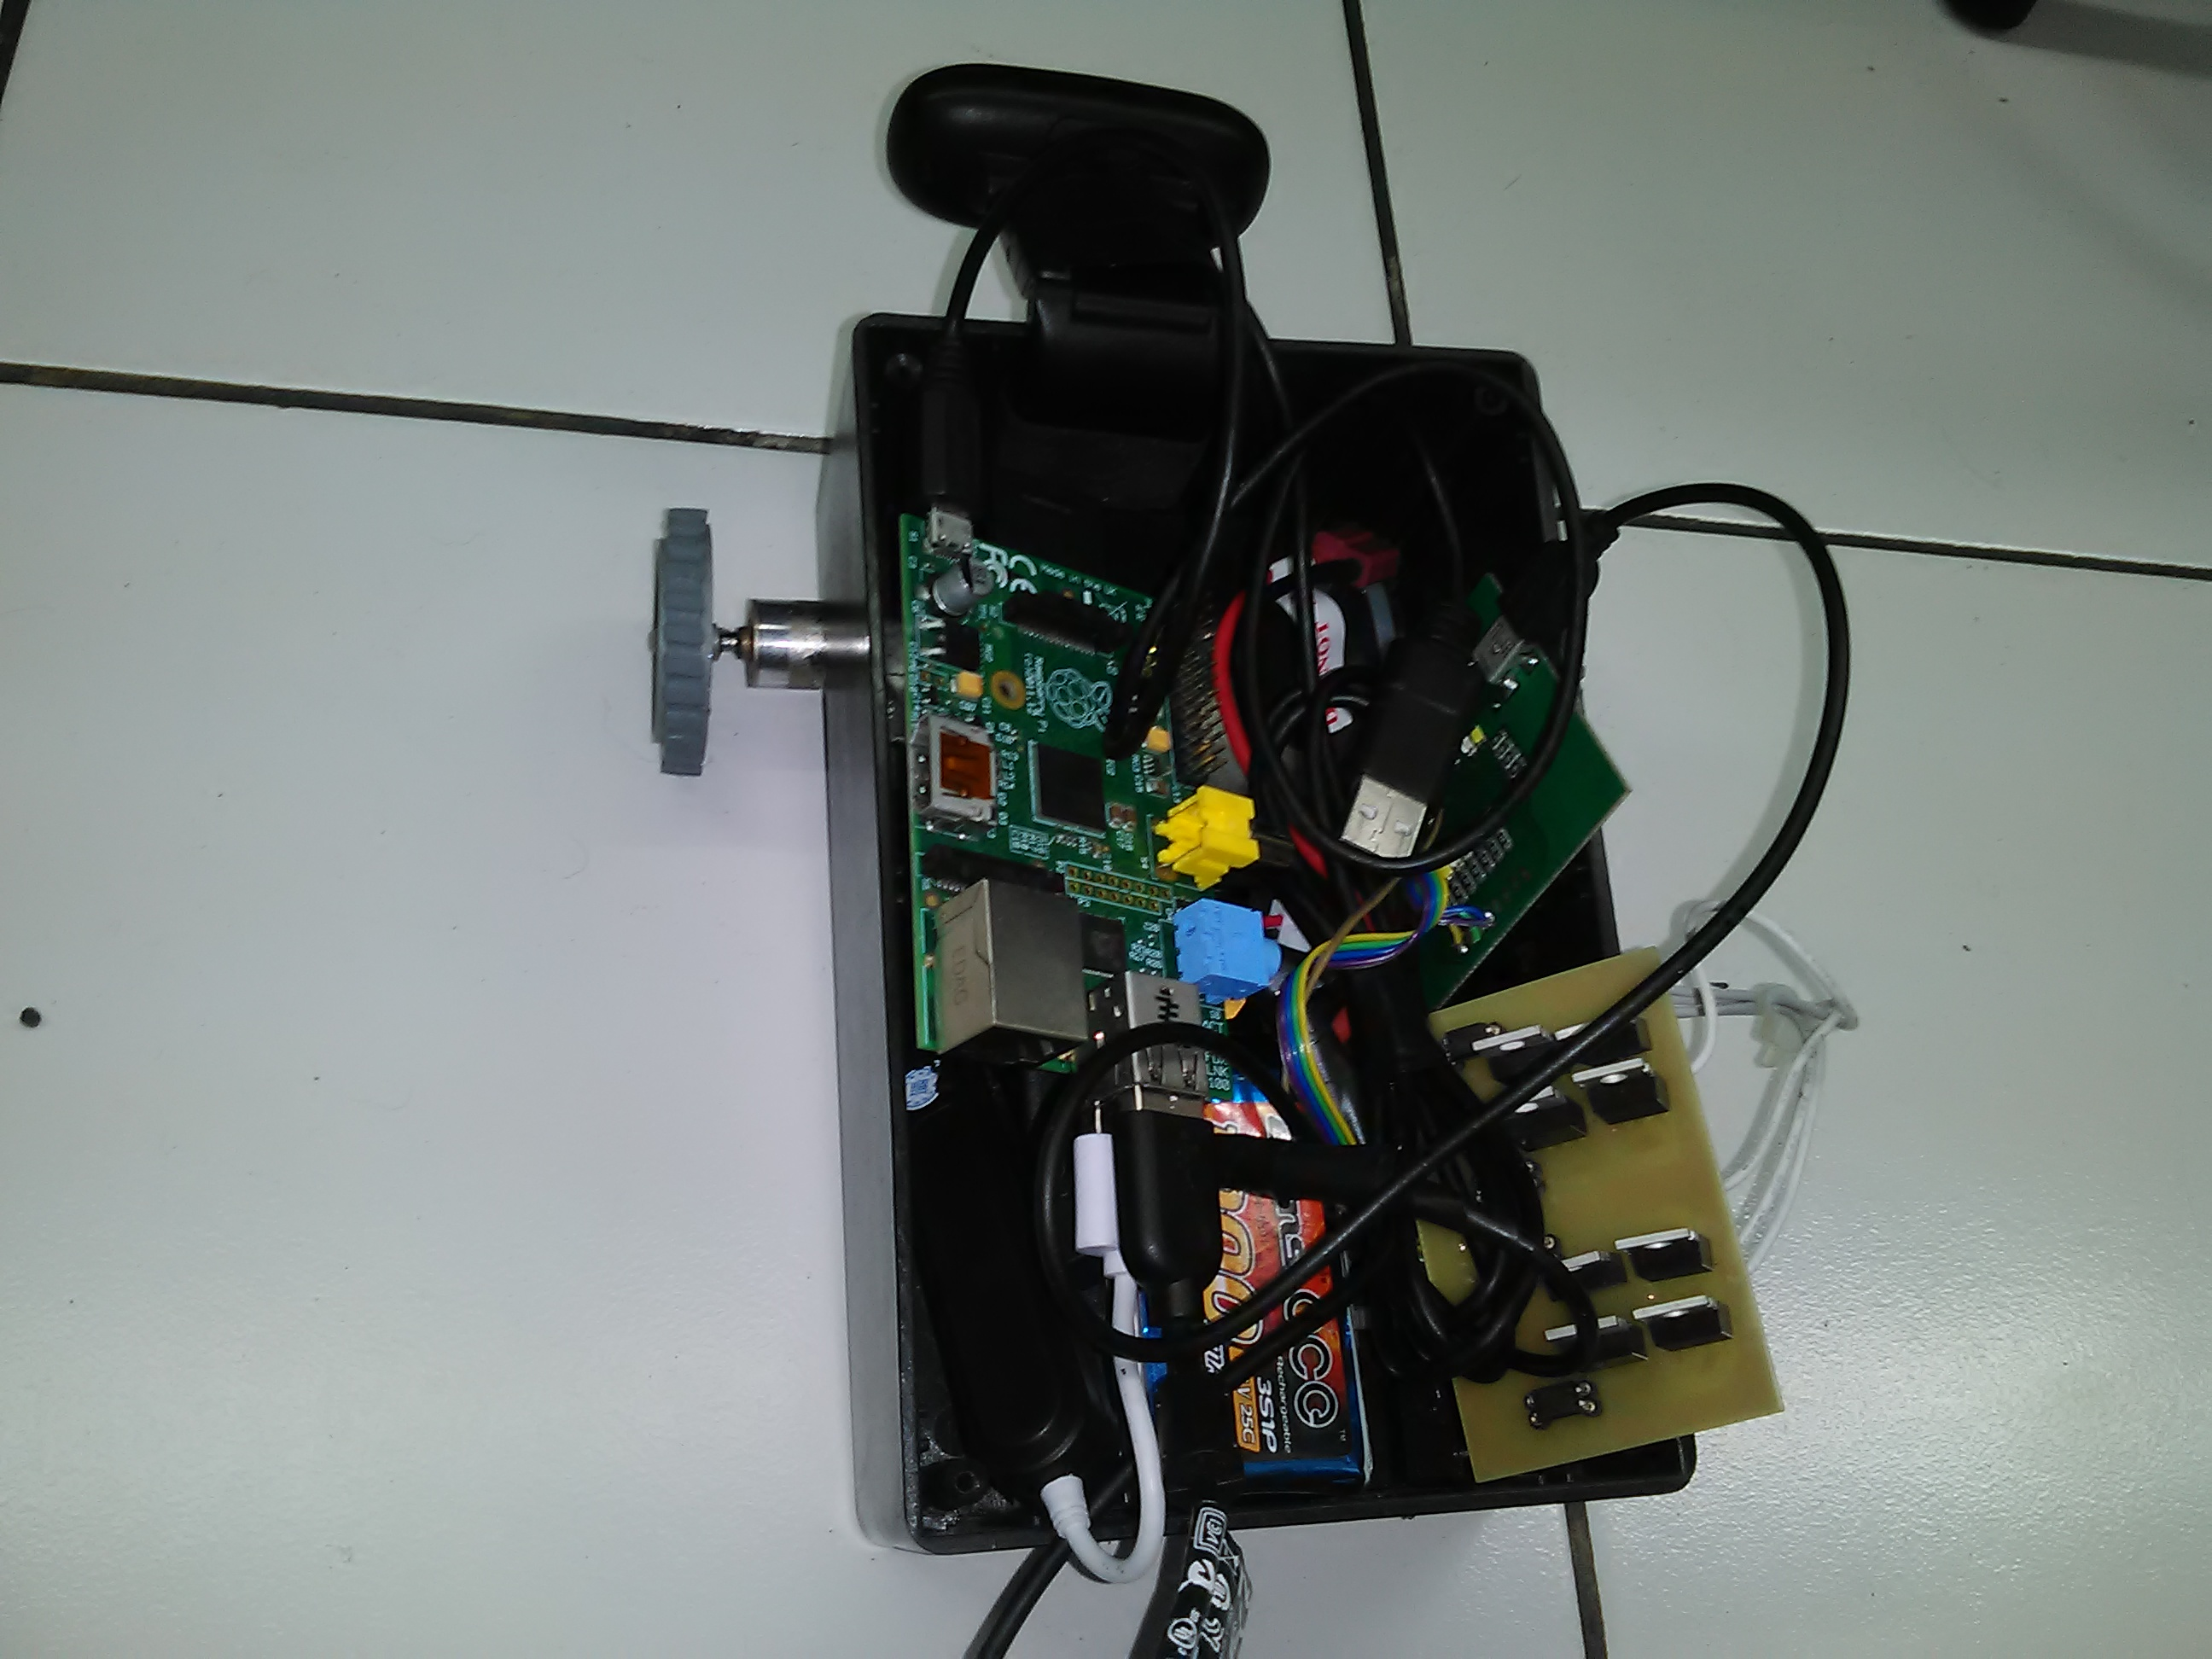
\includegraphics[width=200pt]{full}\\
  \end{center}
  
  \subsection{Perancangan Sistem}
  Secara global alur robot ini terdiri dari:\\

  \begin{center}
    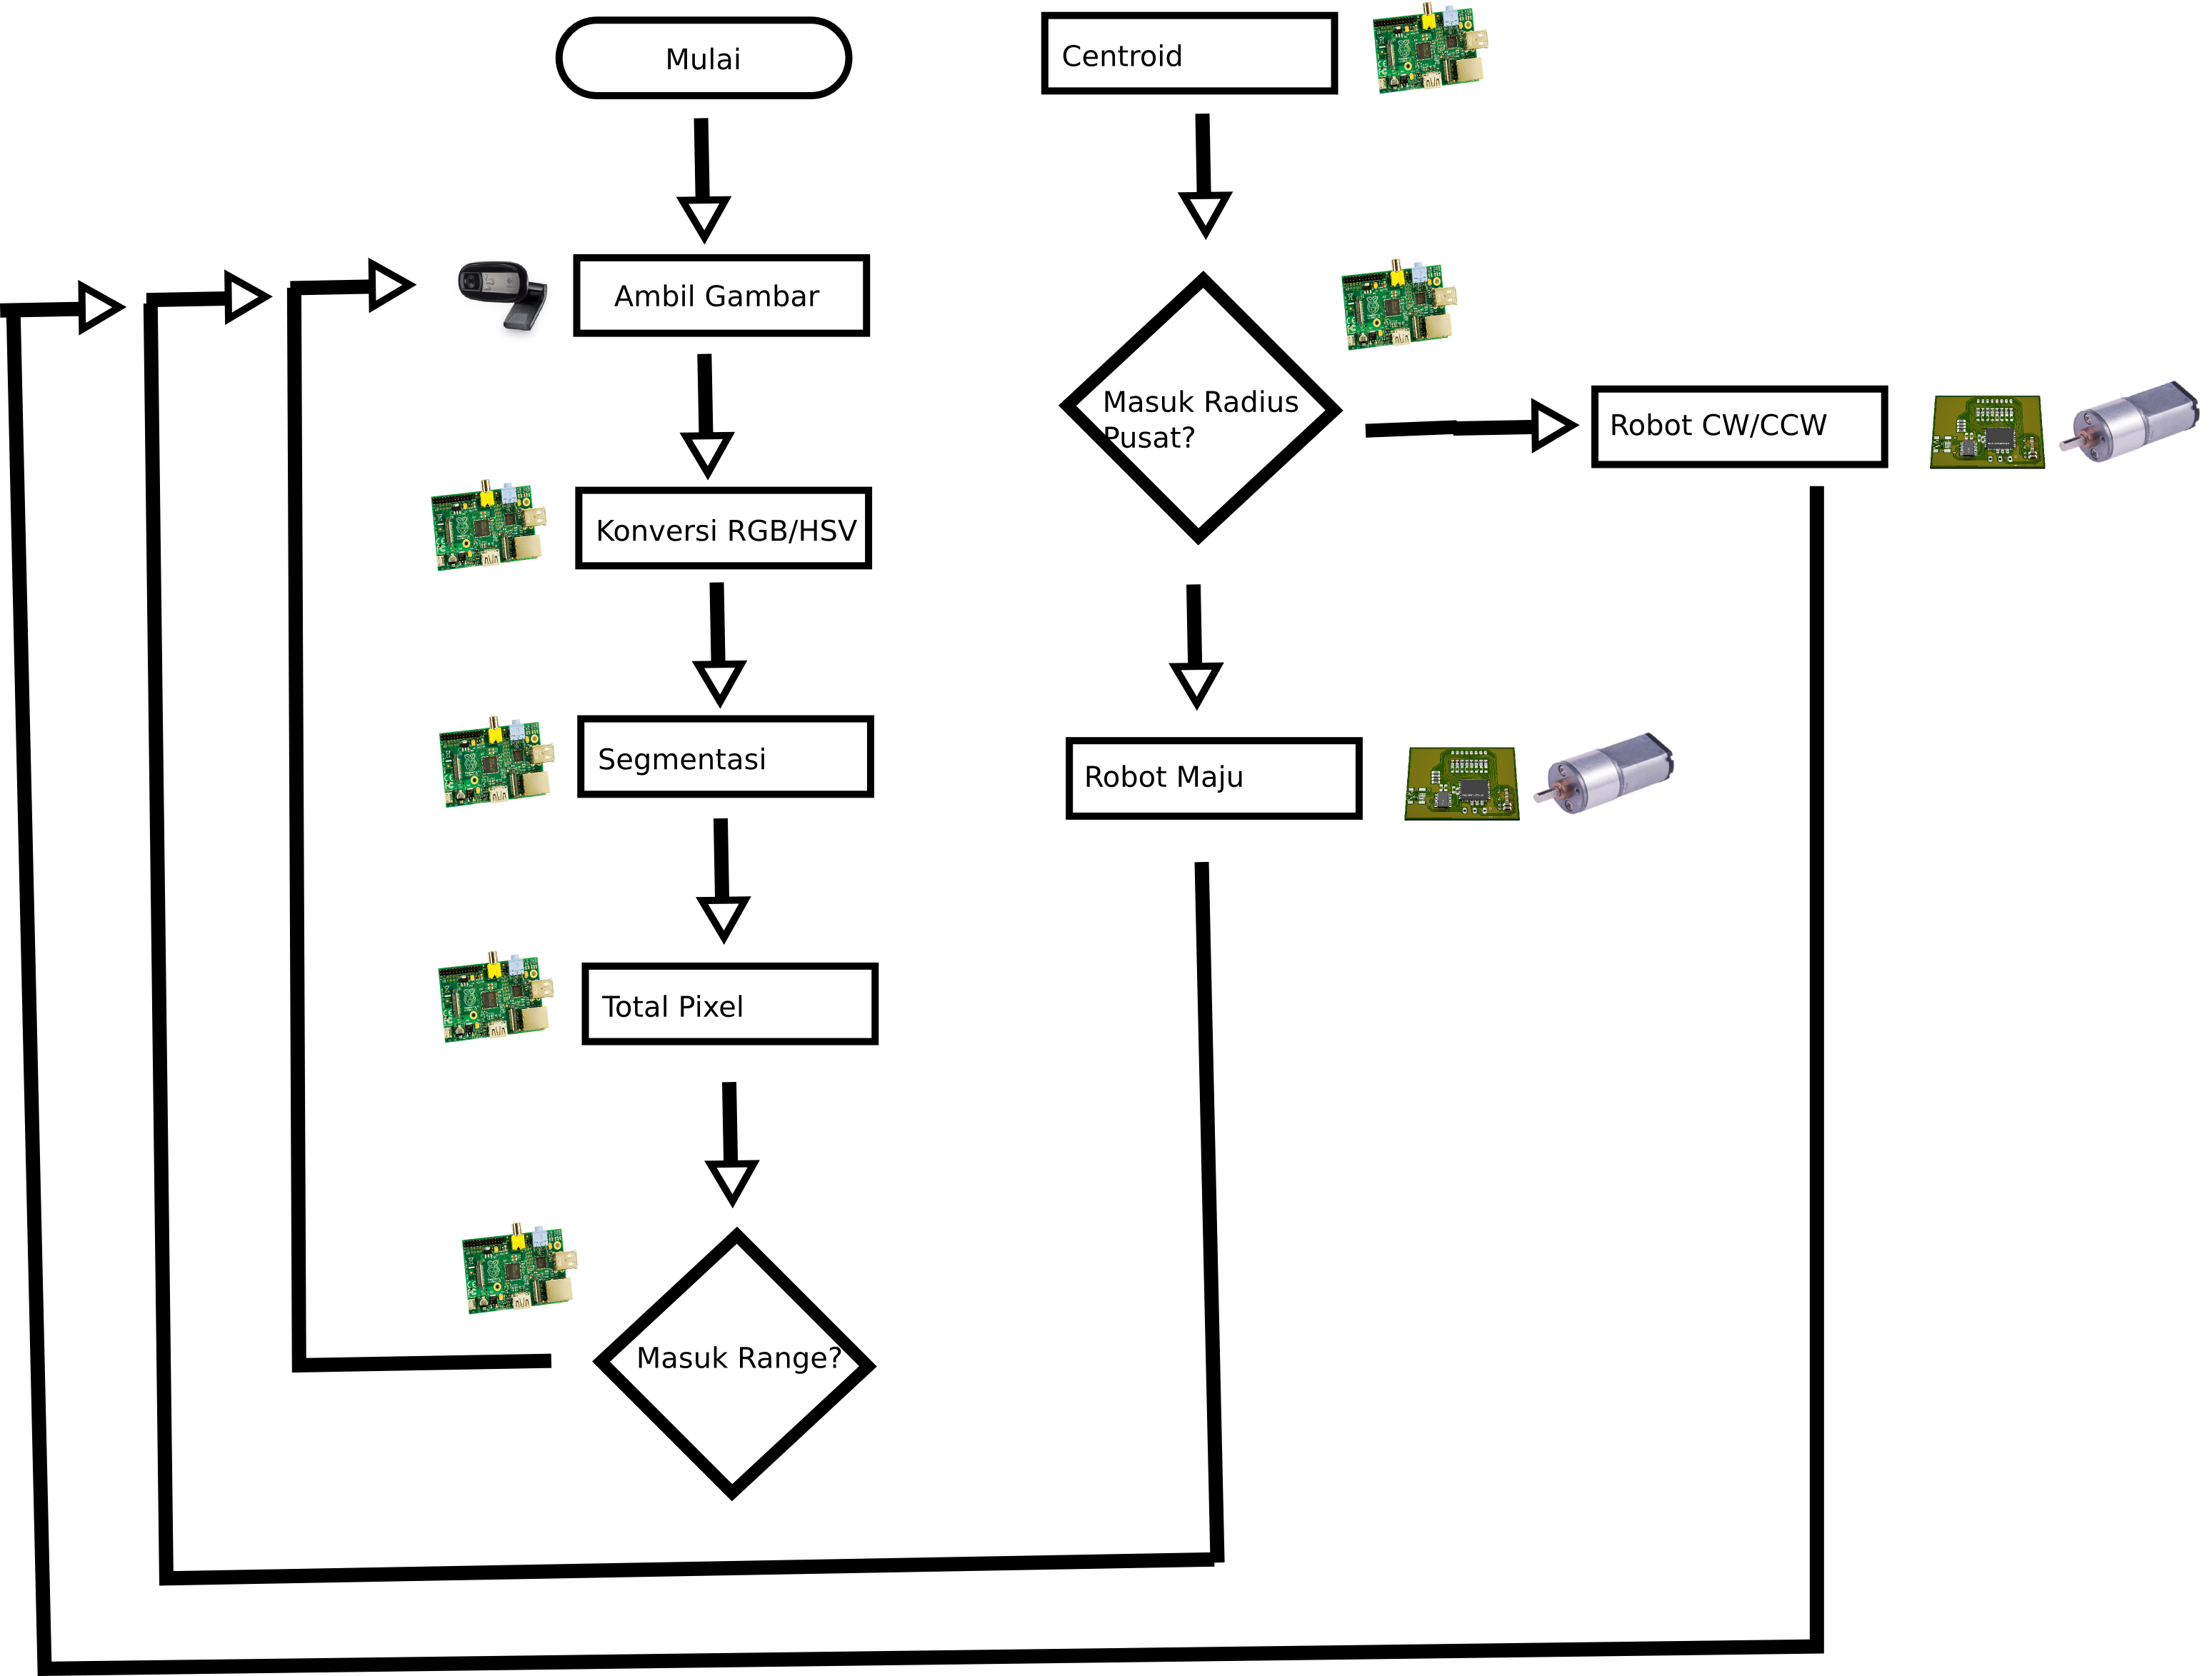
\includegraphics[width=200pt]{process}\\
  \end{center}
  
  Flowchart di atas beserta proses pengolahan citra telah dibentuk menjadi program/software yang dapat dijalankan di CPU.
  Program ini ditulis dengan C/C++ dan mampu membaca web camera untuk diolah berdasarkan nilai HSV yang telah ditentukan serta mampu memberi perintah ke Motor Controller.
  
  \begin{center}
    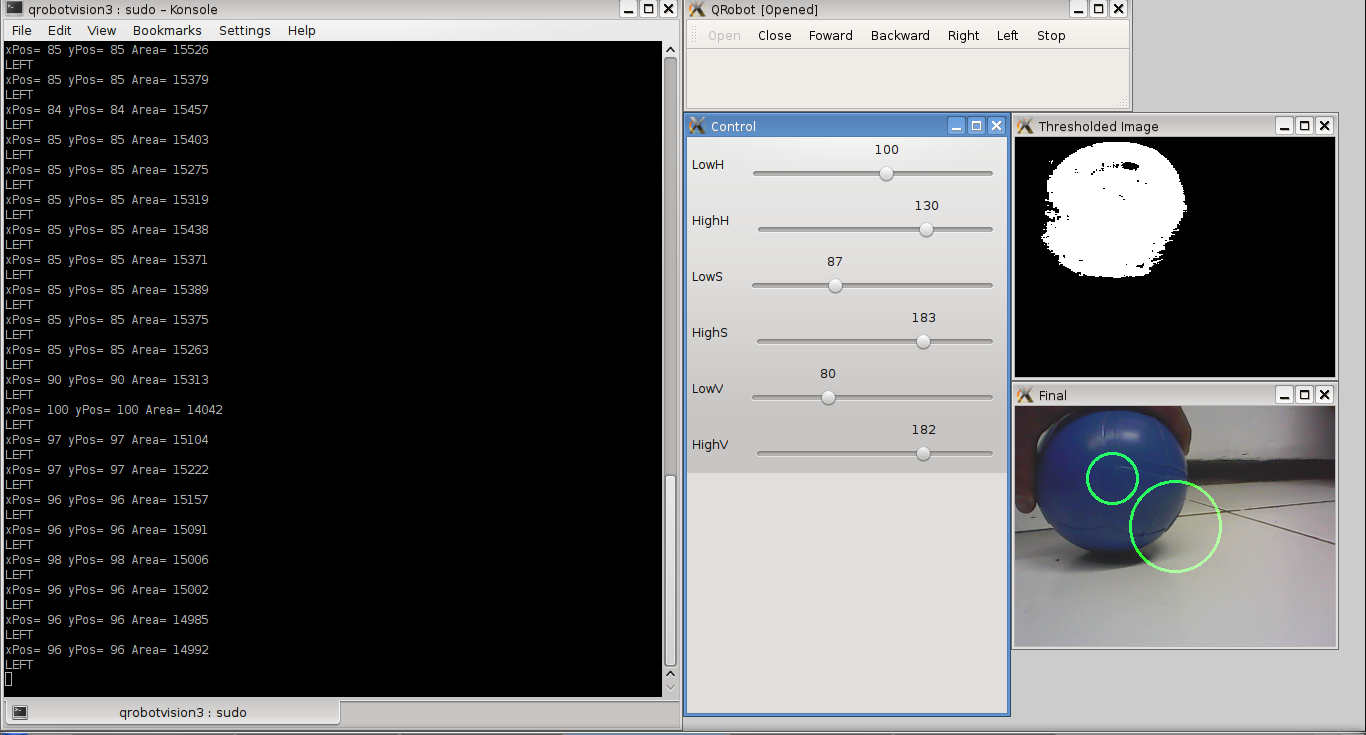
\includegraphics[width=200pt]{softpic}\\
  \end{center}
  
  \section{Hasil}
  
  \subsection{Diagonal Field Of View (FOV)}
  Diagonal Field Of View adalah batas jangkauan kiri dan kanan dari kamera yang dapat ditangkap gambarnya.
  Dalam lembar data dari web camera tertera bahwa FOV yang dimiliki adalah 58 derajat.
  \begin{center}
    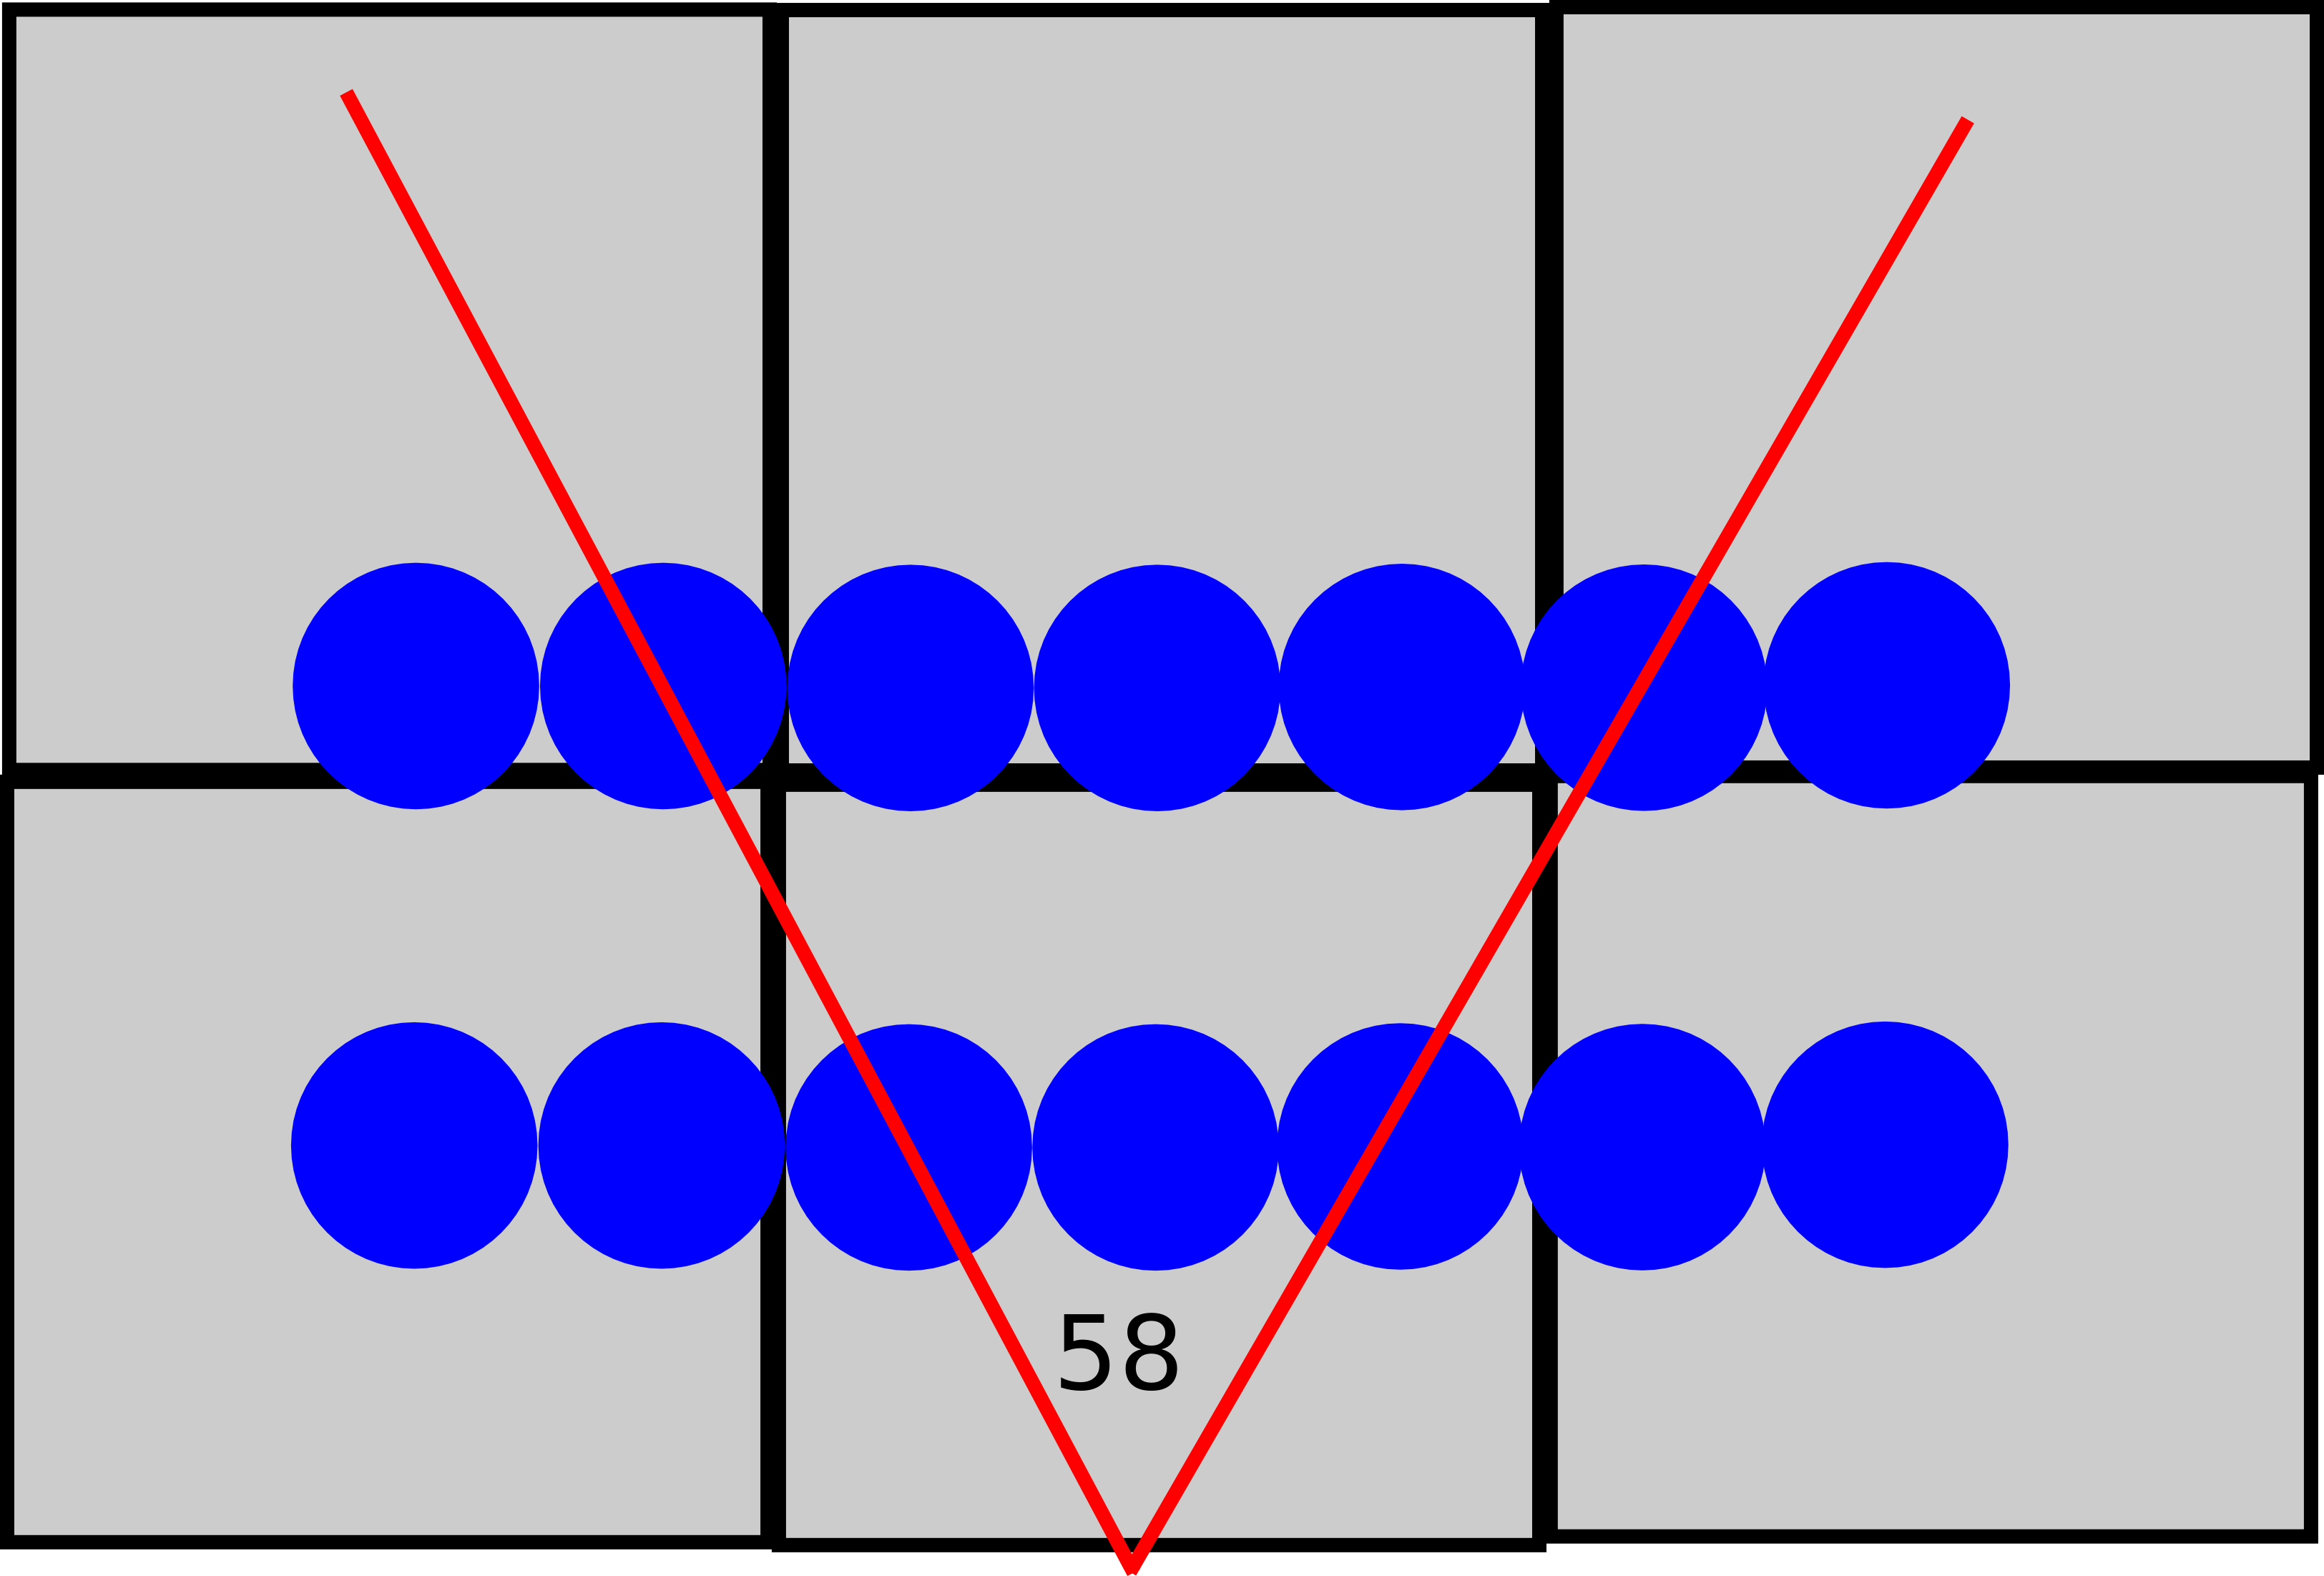
\includegraphics[width=200pt]{fov}\\
  \end{center}
  Untuk memvalidasinya kemudian di ambil gambar seperti skema diatas sehingga didapat sekumpulan gambar yang menunjukkan bahwa Diagonal FOV adalah 58 derajat:
  \begin{center}
    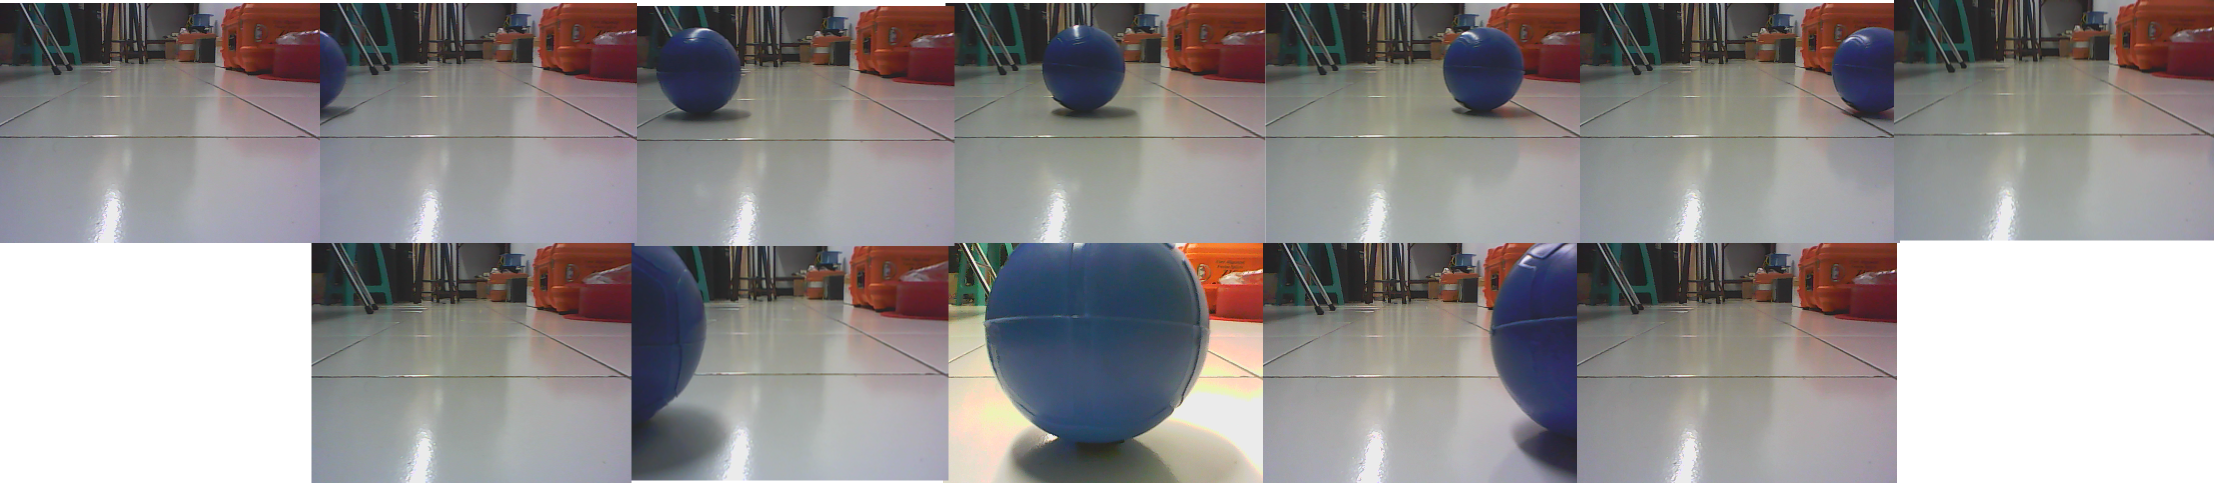
\includegraphics[width=200pt]{data_fov}\\
  \end{center}
  
  \subsection{Range HSV}
  Untuk nilai range pada matrix Hue, telah ditetapkan nilainya oleh pustaka OpenCV.
  Untuk warna biru adalah antara 100-130.
  Sedangkan untuk nilai S dan V didapatkan dengan mengolah gambar mulai dari 0cm hingga 322.5cm dengan kenaikan setiap 15cm diambil 10 gambar maka didapat 440 gambar.
  Setiap gambar diolah agar objek memiliki:\\
  - Jumlah pixel hasil threshold sebanyak mungkin\\
  - Posisi centroid yang masih di radius pusat gambar\\
  Berikut adalah tabel hasil pengolahan 440 gambar teresebut:\\
  \begin{center}
    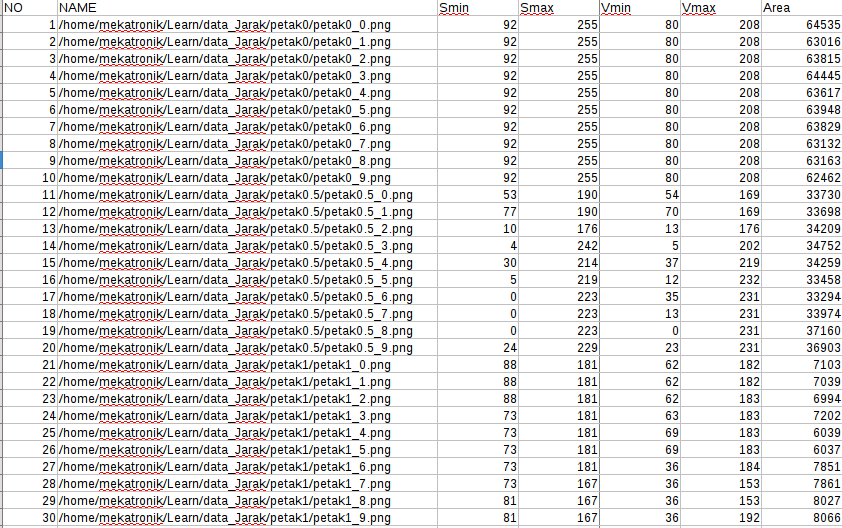
\includegraphics[width=200pt]{data_jarak1}
  \end{center}
  \begin{center}
    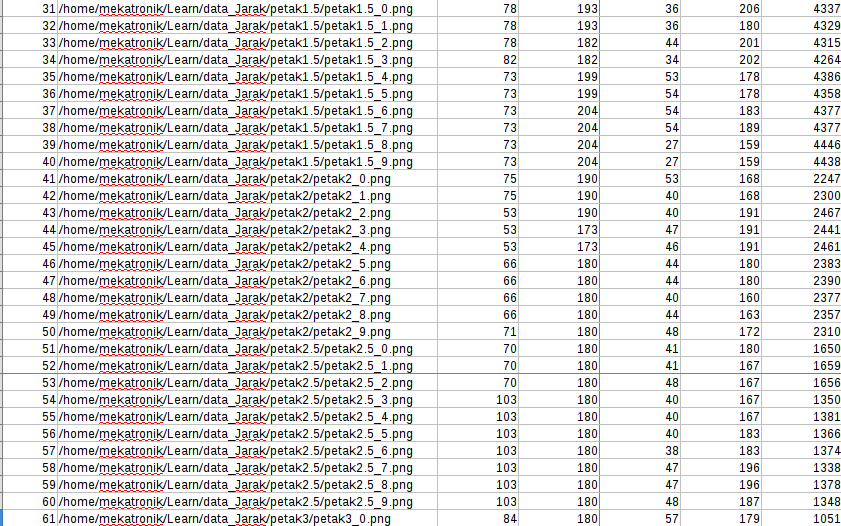
\includegraphics[width=200pt]{data_jarak2}
  \end{center}
  \begin{center}
    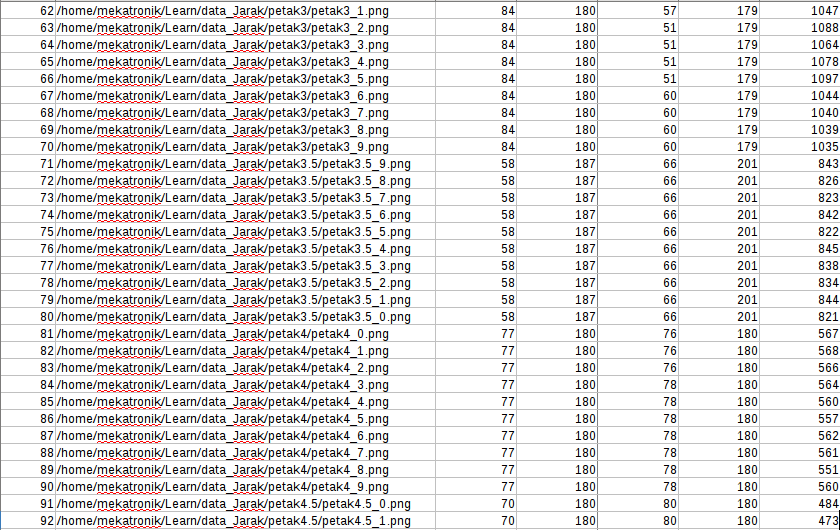
\includegraphics[width=200pt]{data_jarak3}
  \end{center}
  \begin{center}
    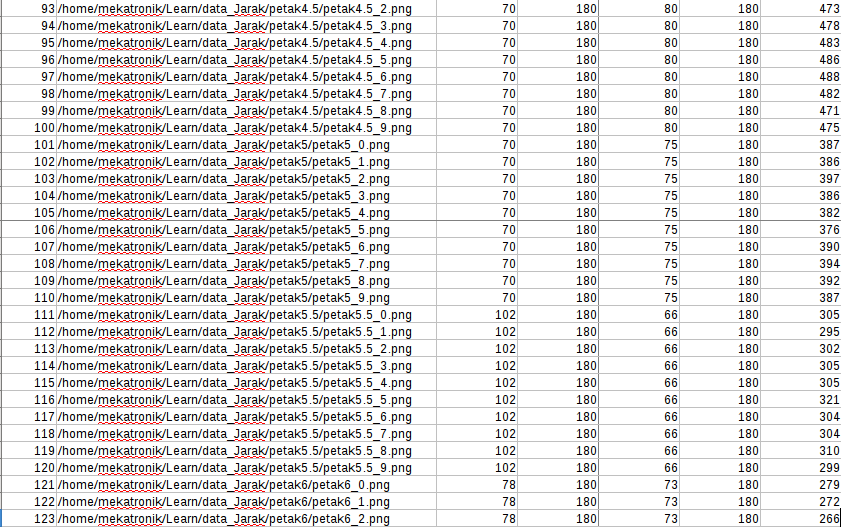
\includegraphics[width=200pt]{data_jarak4}
  \end{center}
  \begin{center}
    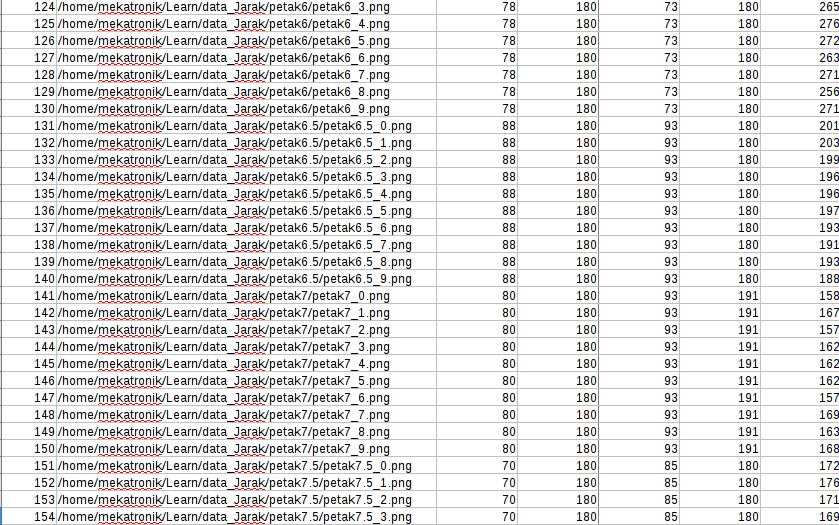
\includegraphics[width=200pt]{data_jarak5}
  \end{center}
  \begin{center}
    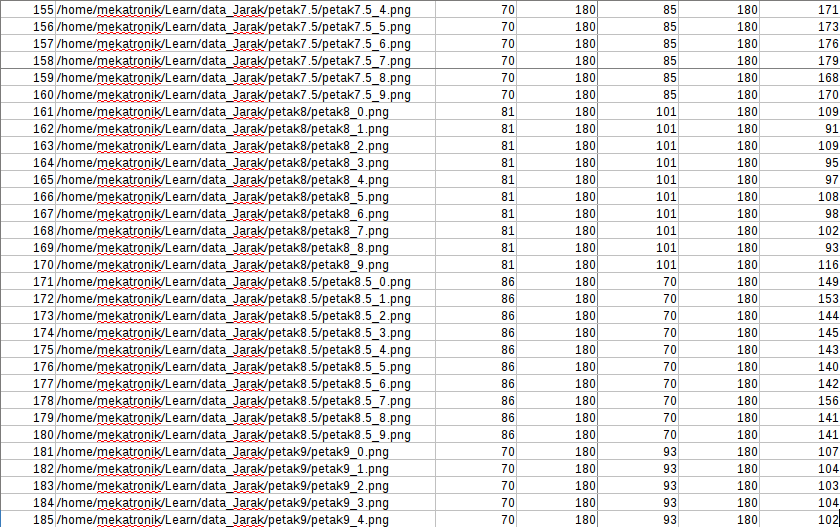
\includegraphics[width=200pt]{data_jarak6}
  \end{center}
  \begin{center}
    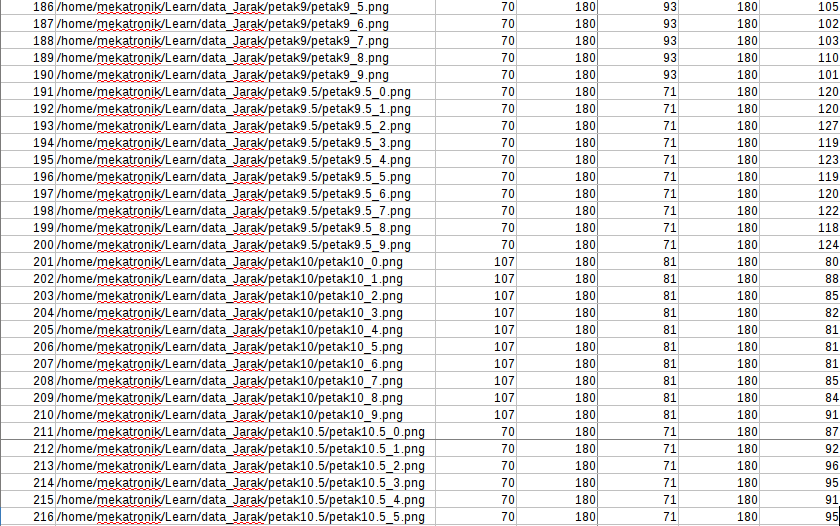
\includegraphics[width=200pt]{data_jarak7}
  \end{center}
  \begin{center}
    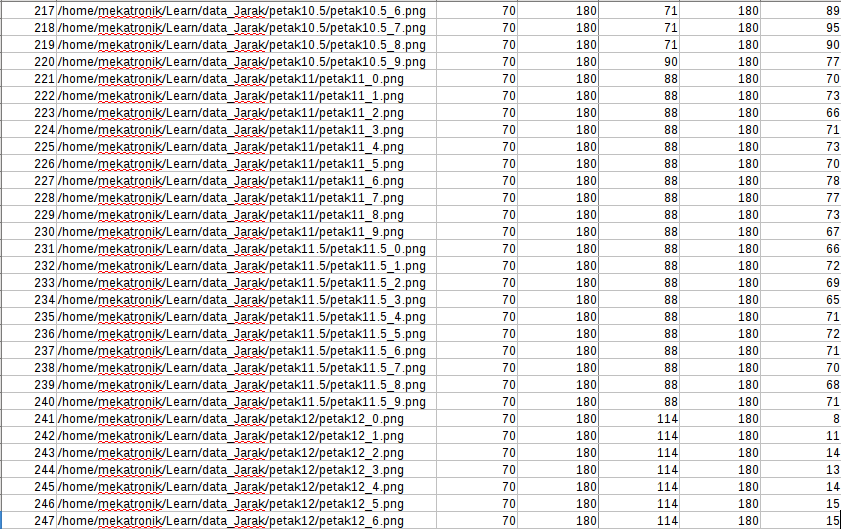
\includegraphics[width=200pt]{data_jarak8}
  \end{center}
  \begin{center}
    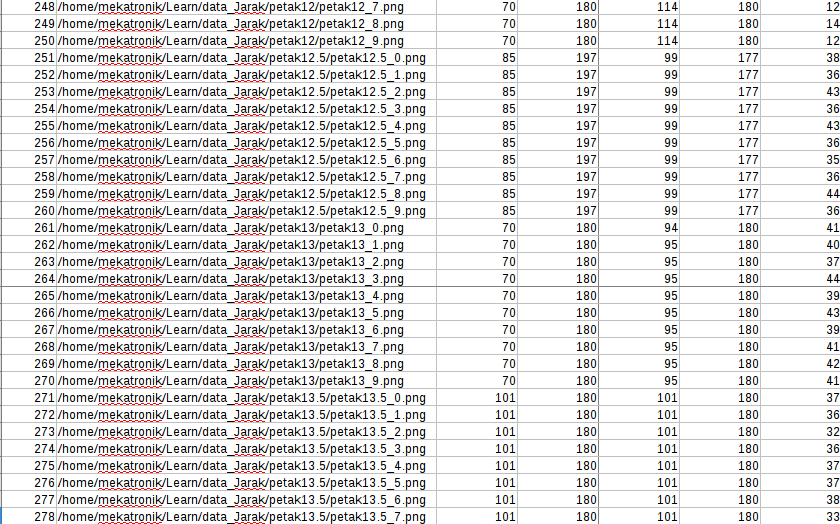
\includegraphics[width=200pt]{data_jarak9}
  \end{center}
  \begin{center}
    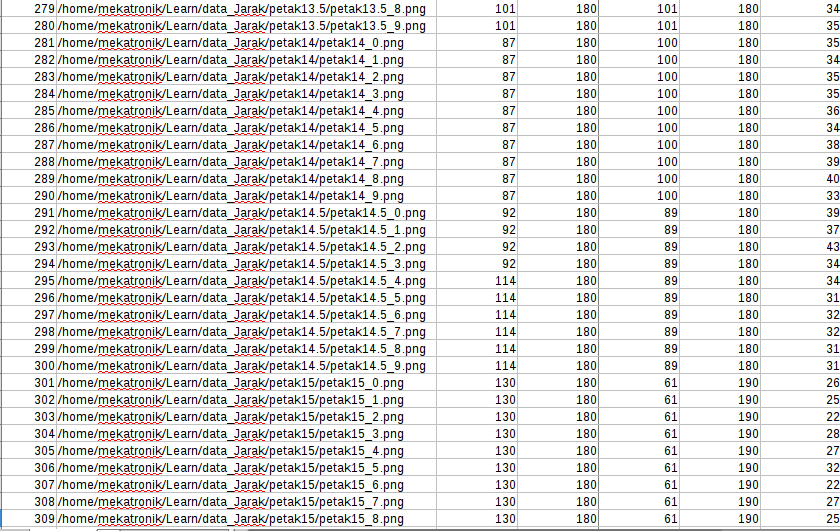
\includegraphics[width=200pt]{data_jarak10}
  \end{center}
  \begin{center}
    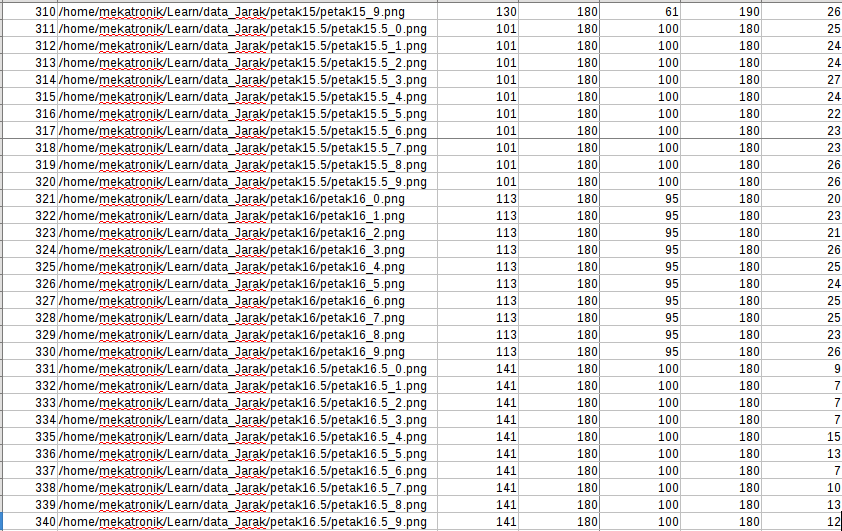
\includegraphics[width=200pt]{data_jarak11}
  \end{center}
  \begin{center}
    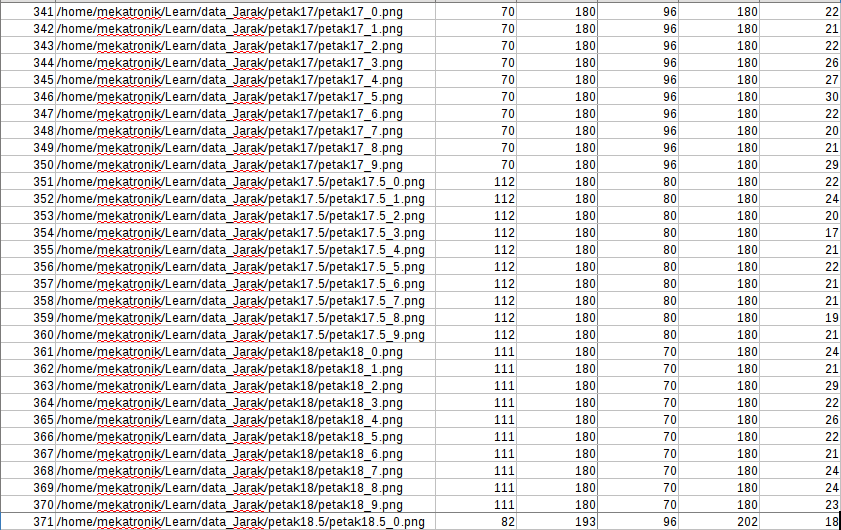
\includegraphics[width=200pt]{data_jarak12}
  \end{center}
  \begin{center}
    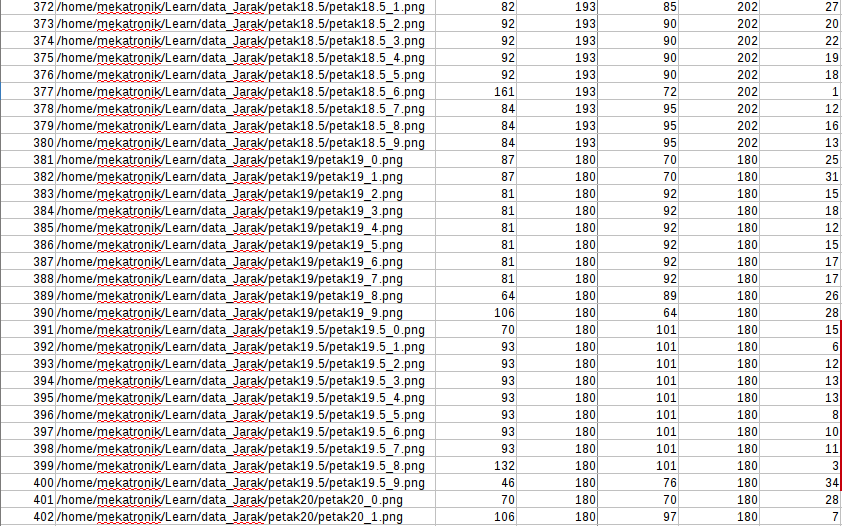
\includegraphics[width=200pt]{data_jarak13}
  \end{center}
  \begin{center}
    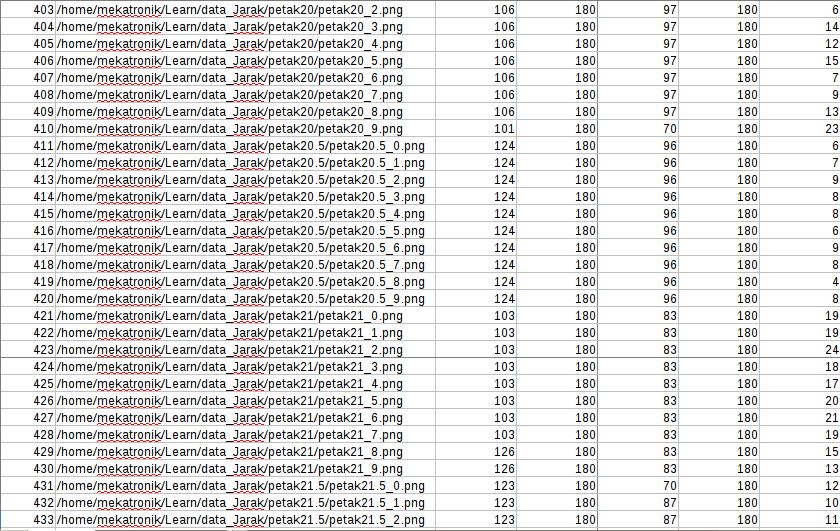
\includegraphics[width=200pt]{data_jarak14}
  \end{center}
  \begin{center}
    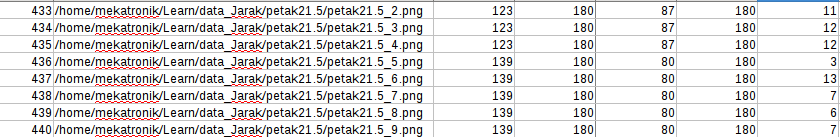
\includegraphics[width=200pt]{data_jarak15}
  \end{center}
  Dengan mengambil rata-rata didapat bahwa nilai Smin adalah 87, Smax adalah 183, Vmin adalah 80, dan Vmax adalah 182.
  Nilai S dan V diatas kemudian digunakan dalam proses threshold.
  Apabila menggunakan nilai S dan V diatas, objek pada jarak lebih 292.5 cm sudah tidak lagi dapat dapat dibedakan antara pixel objek maupun pixel noise karena ukuran pixel objek relatif kecil.
  Kemudian nilai batas bawah dan atas jumlah pixel yang diambil adalah 31 dan 22500.
  
  \subsection{Uji Dinamis}
  Uji Dinamis adalah pengujian robot dengan berjalan.
  Pengujian ini dilakukan untuk mendapatkan hasil eksperimen dari:\\
  - Kecepatan robot untuk menjangkau jarak terjauh.\\
  - Kemampuan robot memilih warna.\\
  Dalam Robot menjangkau jarak terjauh yaitu 292.5 diambil 10 kali pengujian maka robot dapat menemukan objek di setiap pengujian dengan waktu rata-rata adalah 1 menit 10 detik.
  Dalam Robot memilih warna, pengujian dilakukan dengan 4 warna yaitu:\\
  - Merah\\
  - Kuning\\
  - Hijau\\
  - Biru\\
  Semua objek tersebut diletakkan di 10 variasi posisi seperti berikut:
  \begin{center}
    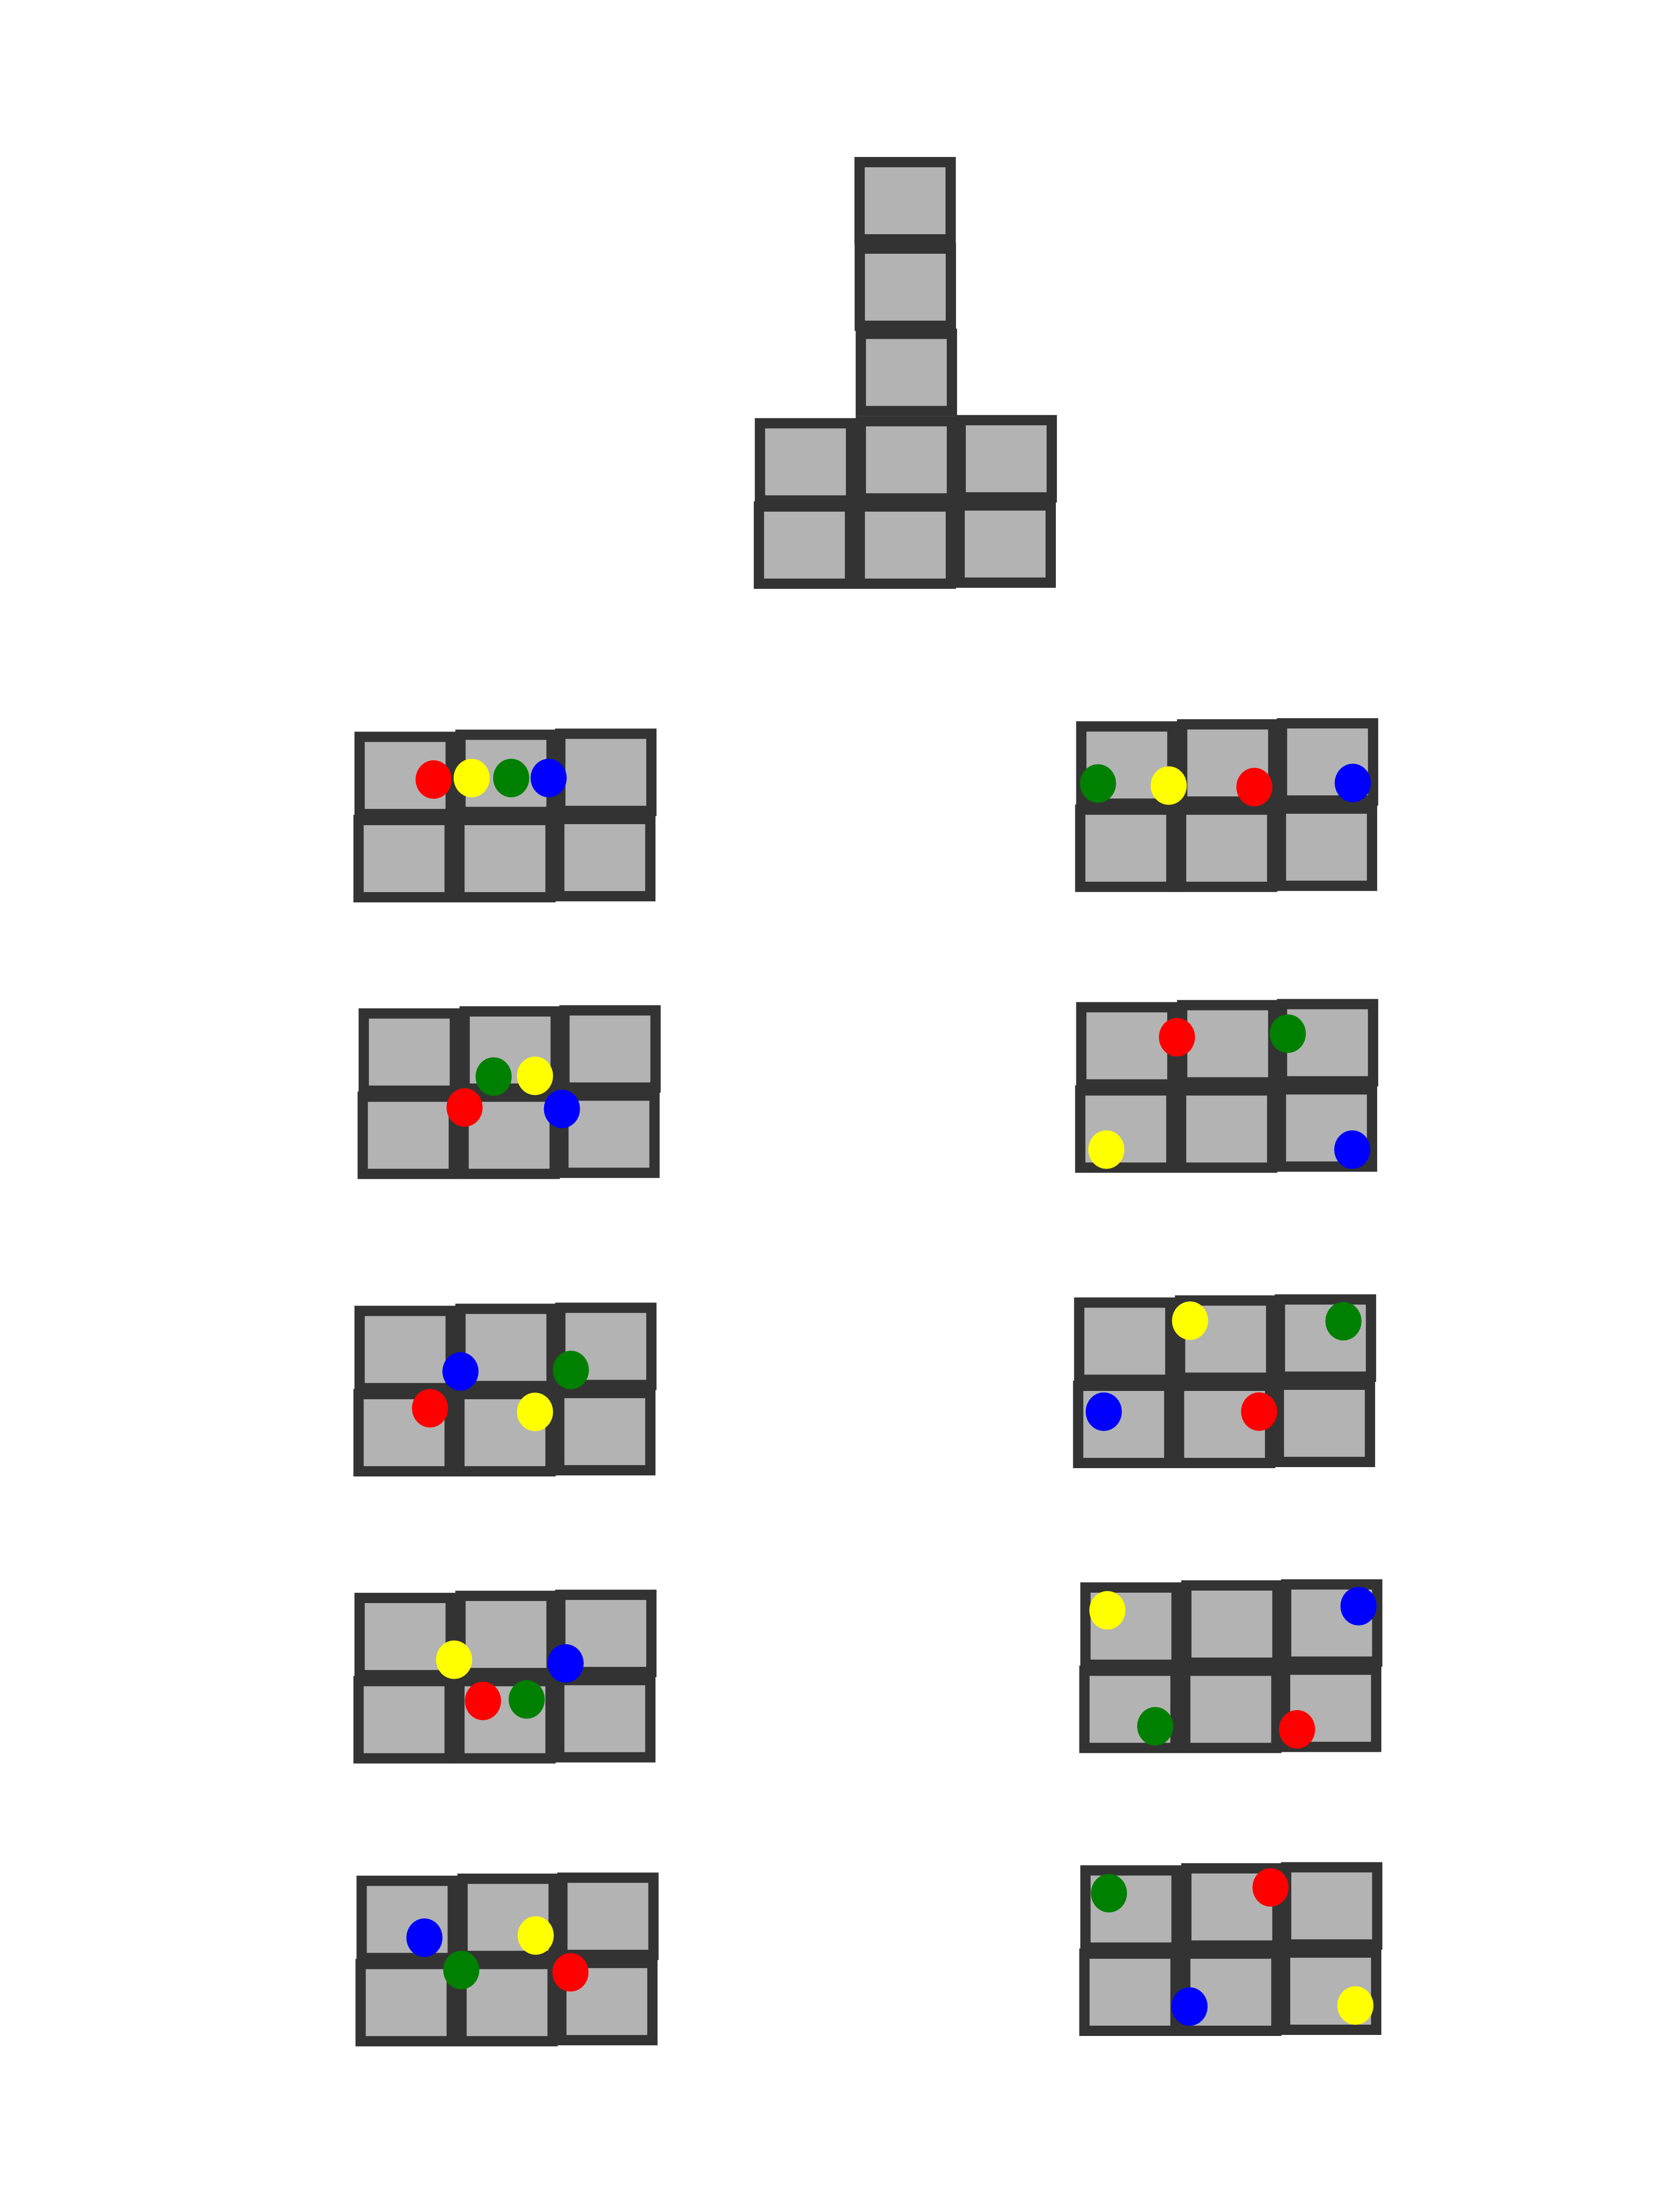
\includegraphics[width=200pt]{uji_warna}
  \end{center}
  Dalam pengujian 10 variasi tersebut robot dapat mendekati setiap bola dengan warna yang telah ditentukan.
  
\end{document}
